\section{Singular Perturbation}
\begin{frame}{Existence of Singularity}
  \begin{figure}[htbp]
    \begin{center}
      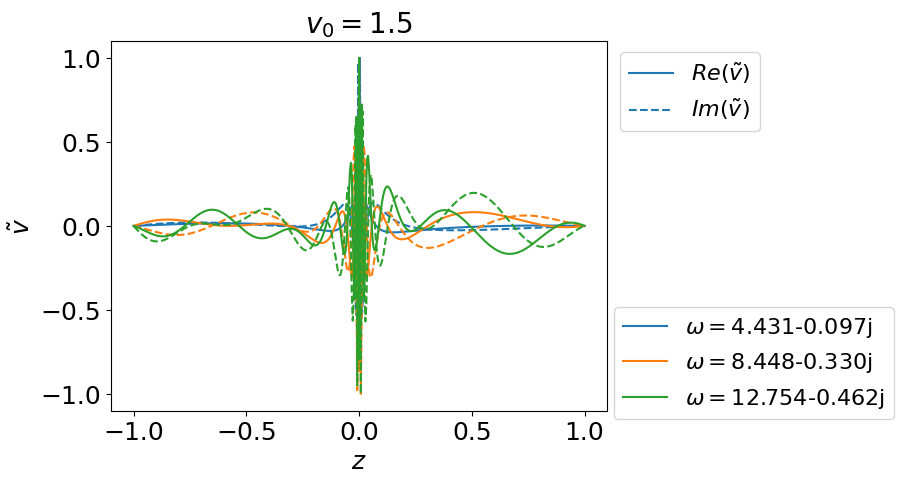
\includegraphics[width=0.95\textwidth]{figures/results-bad-accelerating-v.png}
    \end{center}
    \caption{Spectral method failed to resolve meaningful eigenfunctions (and eigenvalues) due to the existence of the singularity at $z=0$.}
    \label{fig:bad-accelerating-v}
  \end{figure}
\end{frame}

\begin{frame}{Shooting Method}
  \begin{itemize}
    \item Expand $\tilde{v}$ near the singularity using Frobenius method.
    \item Pick up regular solutions and shoot them to the left.
    \item Eigenvalues are found by matching the Dirichlet BC.
  \end{itemize}
  \begin{figure}[htbp]
    \begin{center}
      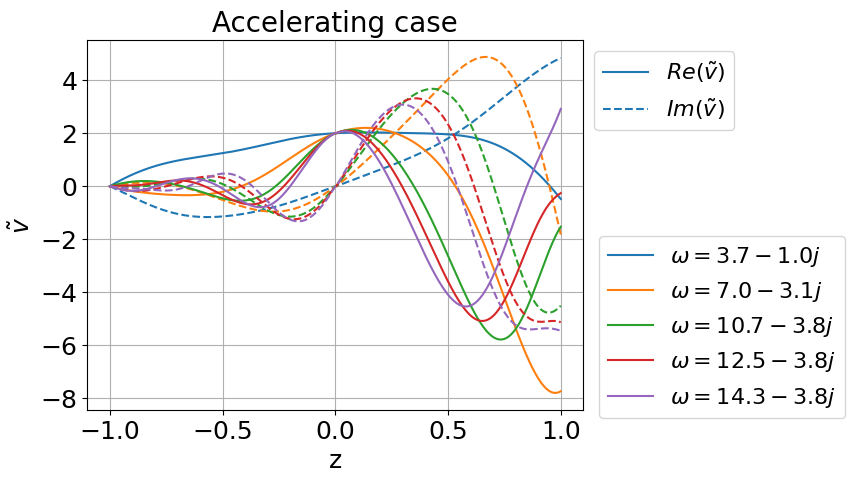
\includegraphics[width=0.7\textwidth]{figures/results-accelerating-v.png}
    \end{center}
    \caption{The solutions crosses the singular point smoothly. All modes are stable.}
    \label{fig:good-accelerating-v}
  \end{figure}
\end{frame}
